\documentclass{beamer}

% Modern theme: Metropolis
\usetheme{metropolis}

% Packages and configurations
\usepackage{graphicx}
\usepackage{amsmath}
\usepackage{courier}
\usepackage{fontspec} % For external fonts
\usepackage{tikz}

% Font for a more modern style (Fira Sans or Roboto)
\setsansfont{Fira Sans} % Ensure it's installed

% Color definitions
\definecolor{myBlue}{RGB}{0, 51, 102} % Dark blue for titles
\definecolor{myAccent}{RGB}{0, 102, 204} % Accent blue for key elements
\definecolor{myBackground}{RGB}{240, 248, 255} % Light background
\definecolor{myGray}{RGB}{200, 200, 200} % Light gray for secondary backgrounds

% Title and author
\title{\textcolor{myBlue}{Preprocessing Automation with Qwen2.5}}
\author{F. Messina, F. Nocella, N. Cherchi}
\date{\textcolor{myAccent}{Academic Year 2024/2025}}

\begin{document}

% Title slide
\begin{frame}[plain]
    \titlepage
\end{frame}

% % Slide: Introduction to the Problem
% \begin{frame}{Introduction to the Problem}
%     \textbf{\textcolor{myBlue}{The Challenge of Data Preprocessing}}
%     \vspace{0.3cm}
%     \begin{itemize}
%         \item \textbf{Data Growth}: Massive data from sources like customer interactions and IoT sensors requires streamlined management for competitive insights.
%         \item \textbf{\textcolor{myAccent}{Data Quality Issues}}: Raw data is often incomplete or inconsistent, demanding extensive cleaning and preparation before analysis.
%         \item \textbf{\textcolor{myAccent}{Manual Preprocessing Challenges}}: Current processes are time-consuming, requiring specialized skills to manage complex datasets effectively.
%     \end{itemize}
% \end{frame}

% Slide: Introduction to the Problem
\begin{frame}{Introduction to the Problem}
    \textbf{\textcolor{myBlue}{The Challenge of Data Preprocessing}}
    \vspace{0.3cm}
    \begin{itemize}
        \item \textbf{Data Growth}: Massive data from sources like customer interactions and IoT sensors requires streamlined management for competitive insights.
        \item \textbf{\textcolor{myAccent}{Importance of Data in Business}}: High-quality data is a key asset, empowering decision-making, enhancing customer experience, and driving business innovation.
        \item \textbf{{Data Quality Issues}}: Raw data is often incomplete or inconsistent, demanding extensive cleaning and preparation before analysis.
        \item \textbf{\textcolor{myAccent}{Manual Preprocessing Challenges}}: Current processes are time-consuming, requiring specialized skills to manage complex datasets effectively.
    \end{itemize}
\end{frame}


% Slide: Project Goals
\begin{frame}{Project Goals}
    \textbf{\textcolor{myBlue}{Automating Data Preprocessing with Qwen2.5}}
    \vspace{0.3cm}
    \begin{itemize}
        \item \textbf{Objective}: Evaluate Qwen2.5's potential to automate preprocessing, minimizing manual intervention.
        \item \textbf{\textcolor{myAccent}{Expected Benefits}}:
        \begin{itemize}
            \item Reduce time and costs by automating repetitive tasks.
            \item Improve data quality and consistency, enabling scalable, reliable analysis.
        \end{itemize}
    \end{itemize}
\end{frame}



% Business-Driven Application Design
\begin{frame}{Business-Driven Application Design}
    \textbf{\textcolor{myBlue}{Designing an Application for Business Optimization}}
    \vspace{0.3cm}
    \begin{itemize}
        \item \textbf{Model Selection}: Qwen2.5 1.5B, chosen for its speed and efficiency.
        \item \textbf{Two-Level Architecture}:
            \begin{itemize}
                \item \textbf{Logical Level}: Creating a framework for scalable, reusable data preprocessing workflows.
                \item \textbf{Code Generation Level}: Automating the generation of executable code for rapid deployment in business environments.
            \end{itemize}
        \item \textbf{Validation}: Testing on datasets to ensure accuracy and reliability before business integration.
    \end{itemize}
\end{frame}

% Technologies Used
\begin{frame}{Technologies Used}
    \textbf{\textcolor{myBlue}{Core Technologies}}
    \vspace{0.3cm}
    \begin{itemize}
        \item \textbf{Qwen2.5}: Open-source language model for natural language processing, providing secure, scalable, and cost-effective automation solutions for enterprises.
        \item \textbf{Python}: With libraries such as PyTorch, enabling quick deployment and flexibility.
    \end{itemize}
\end{frame}

\begin{frame}{Mockup of the application - 1/2}
    \vspace{0.2cm}
    \begin{figure}
        \centering
        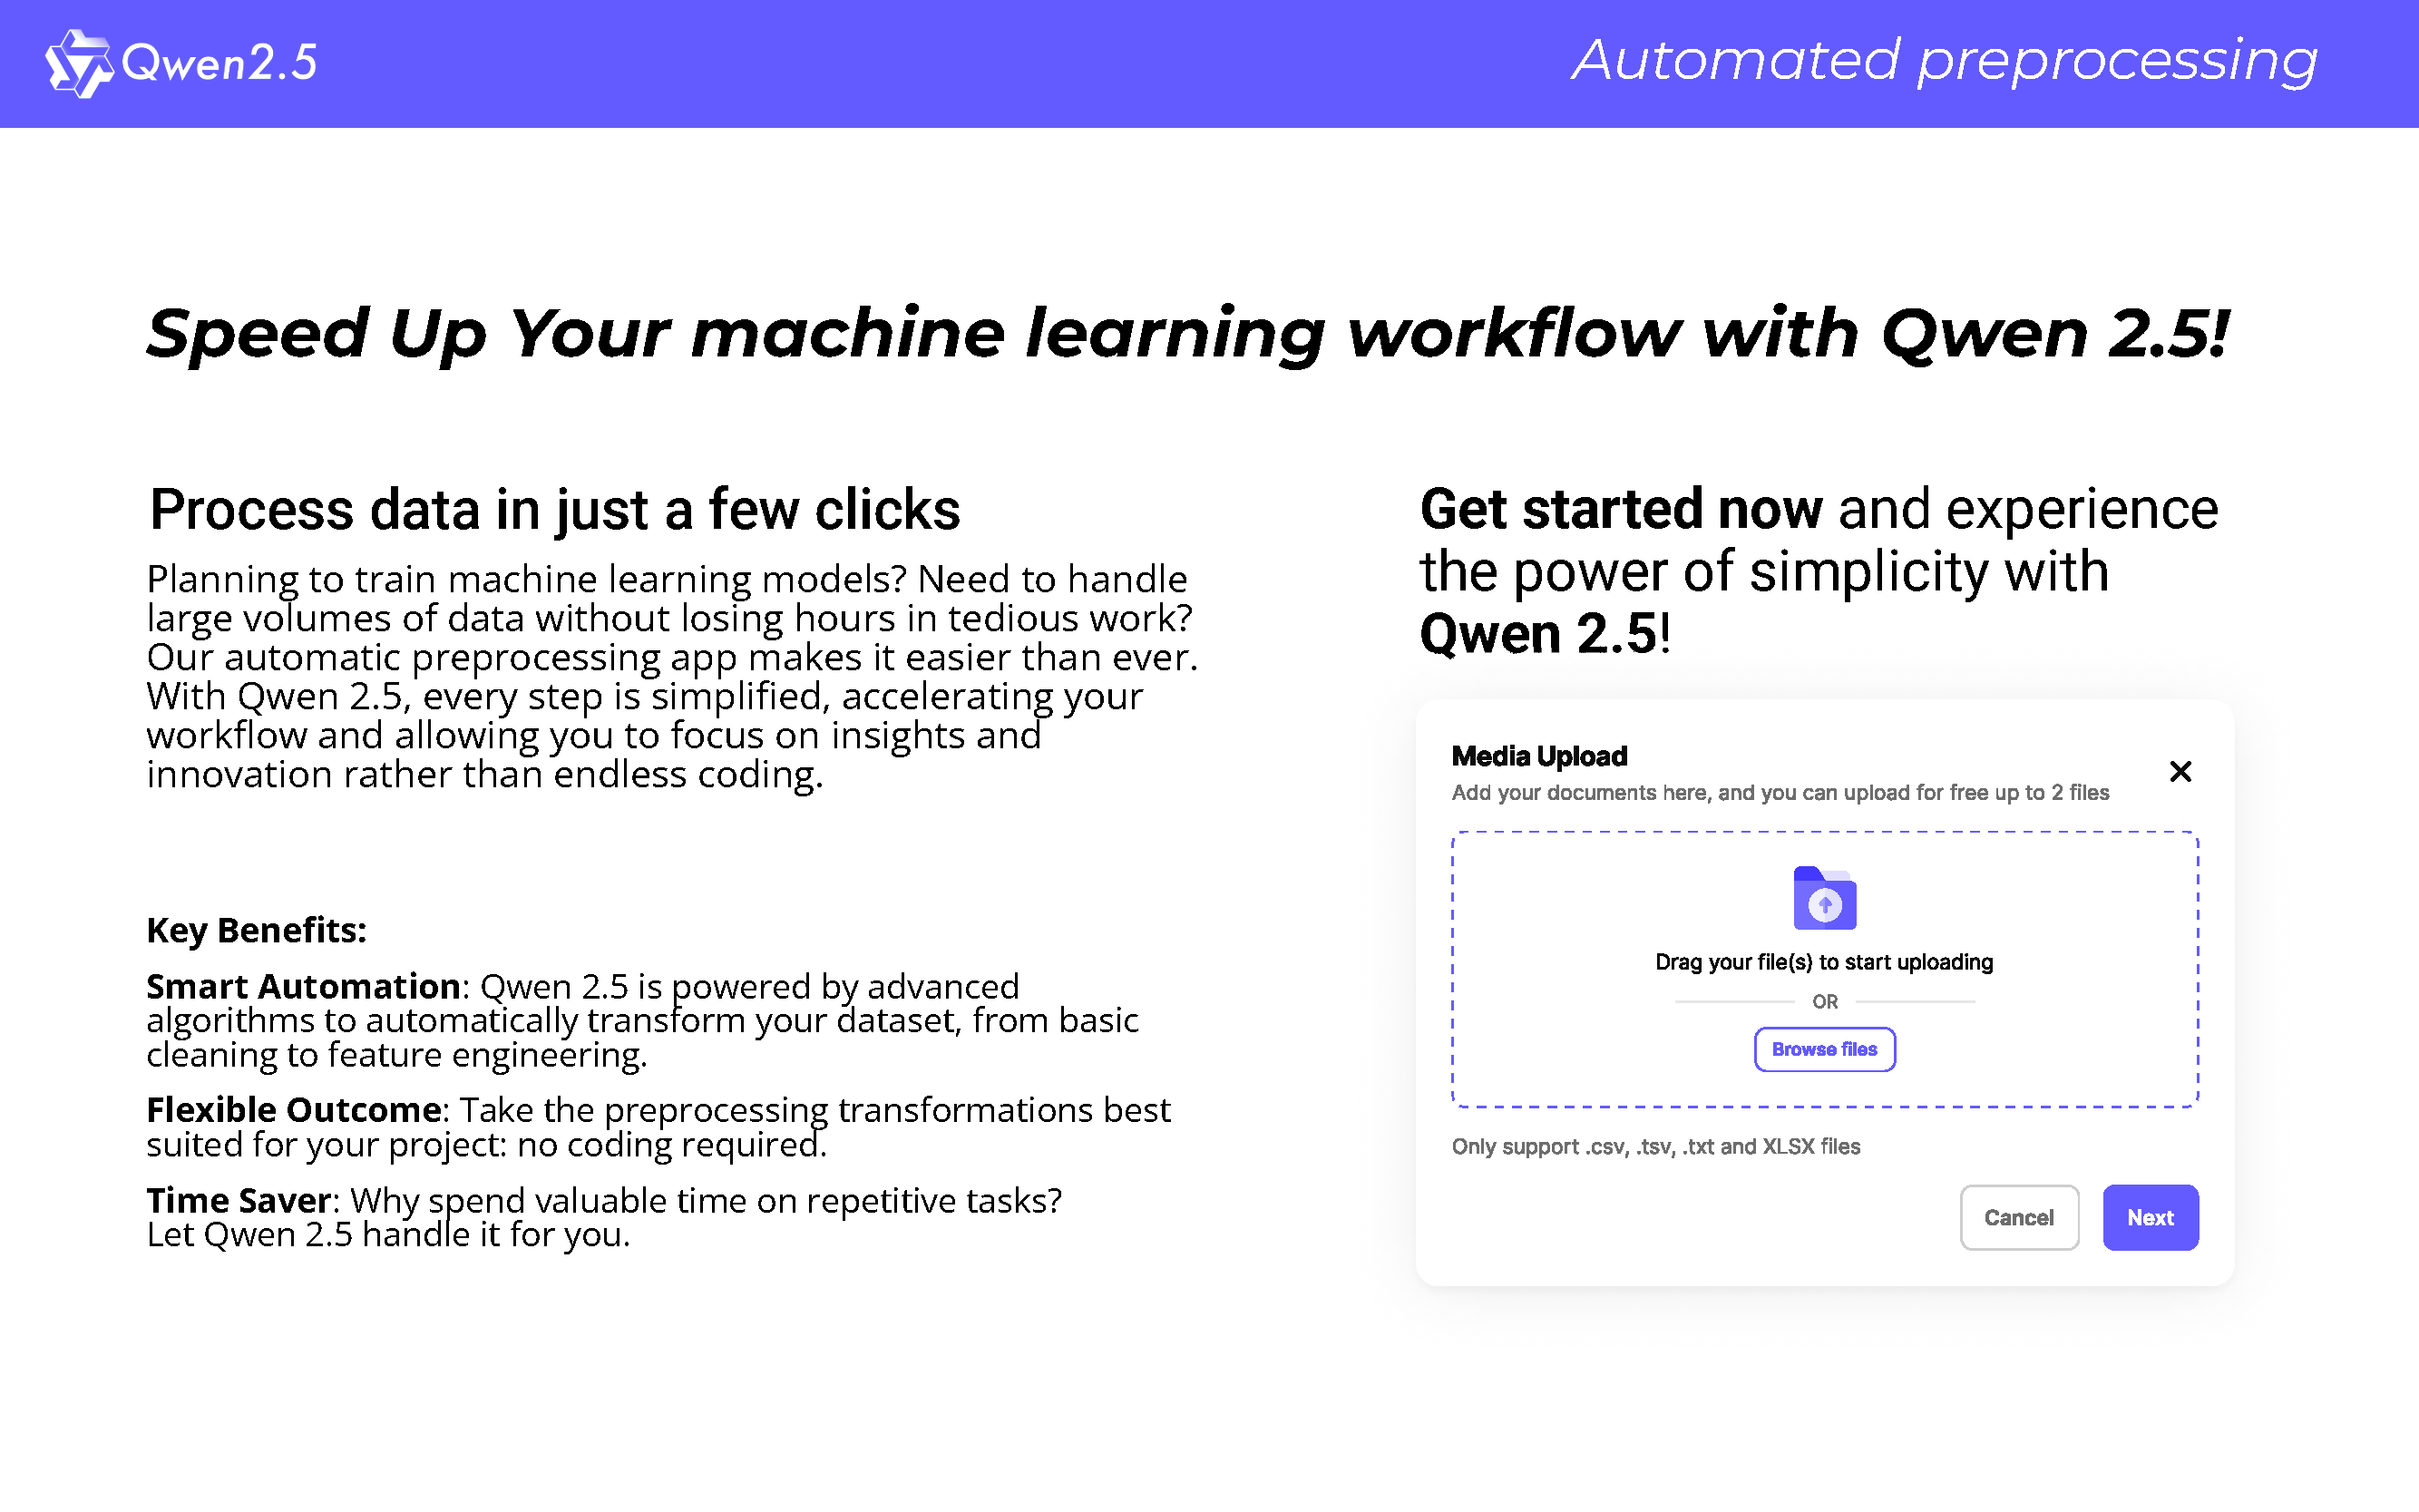
\includegraphics[width=\textwidth]{App_prototipo_1.pdf}
        \caption{Main page of the Qwen2.5 application} 
    \end{figure}
\end{frame}

\begin{frame}{Mockup of the application - 2/2}
    \vspace{0.2cm}
    \begin{figure}
        \centering
        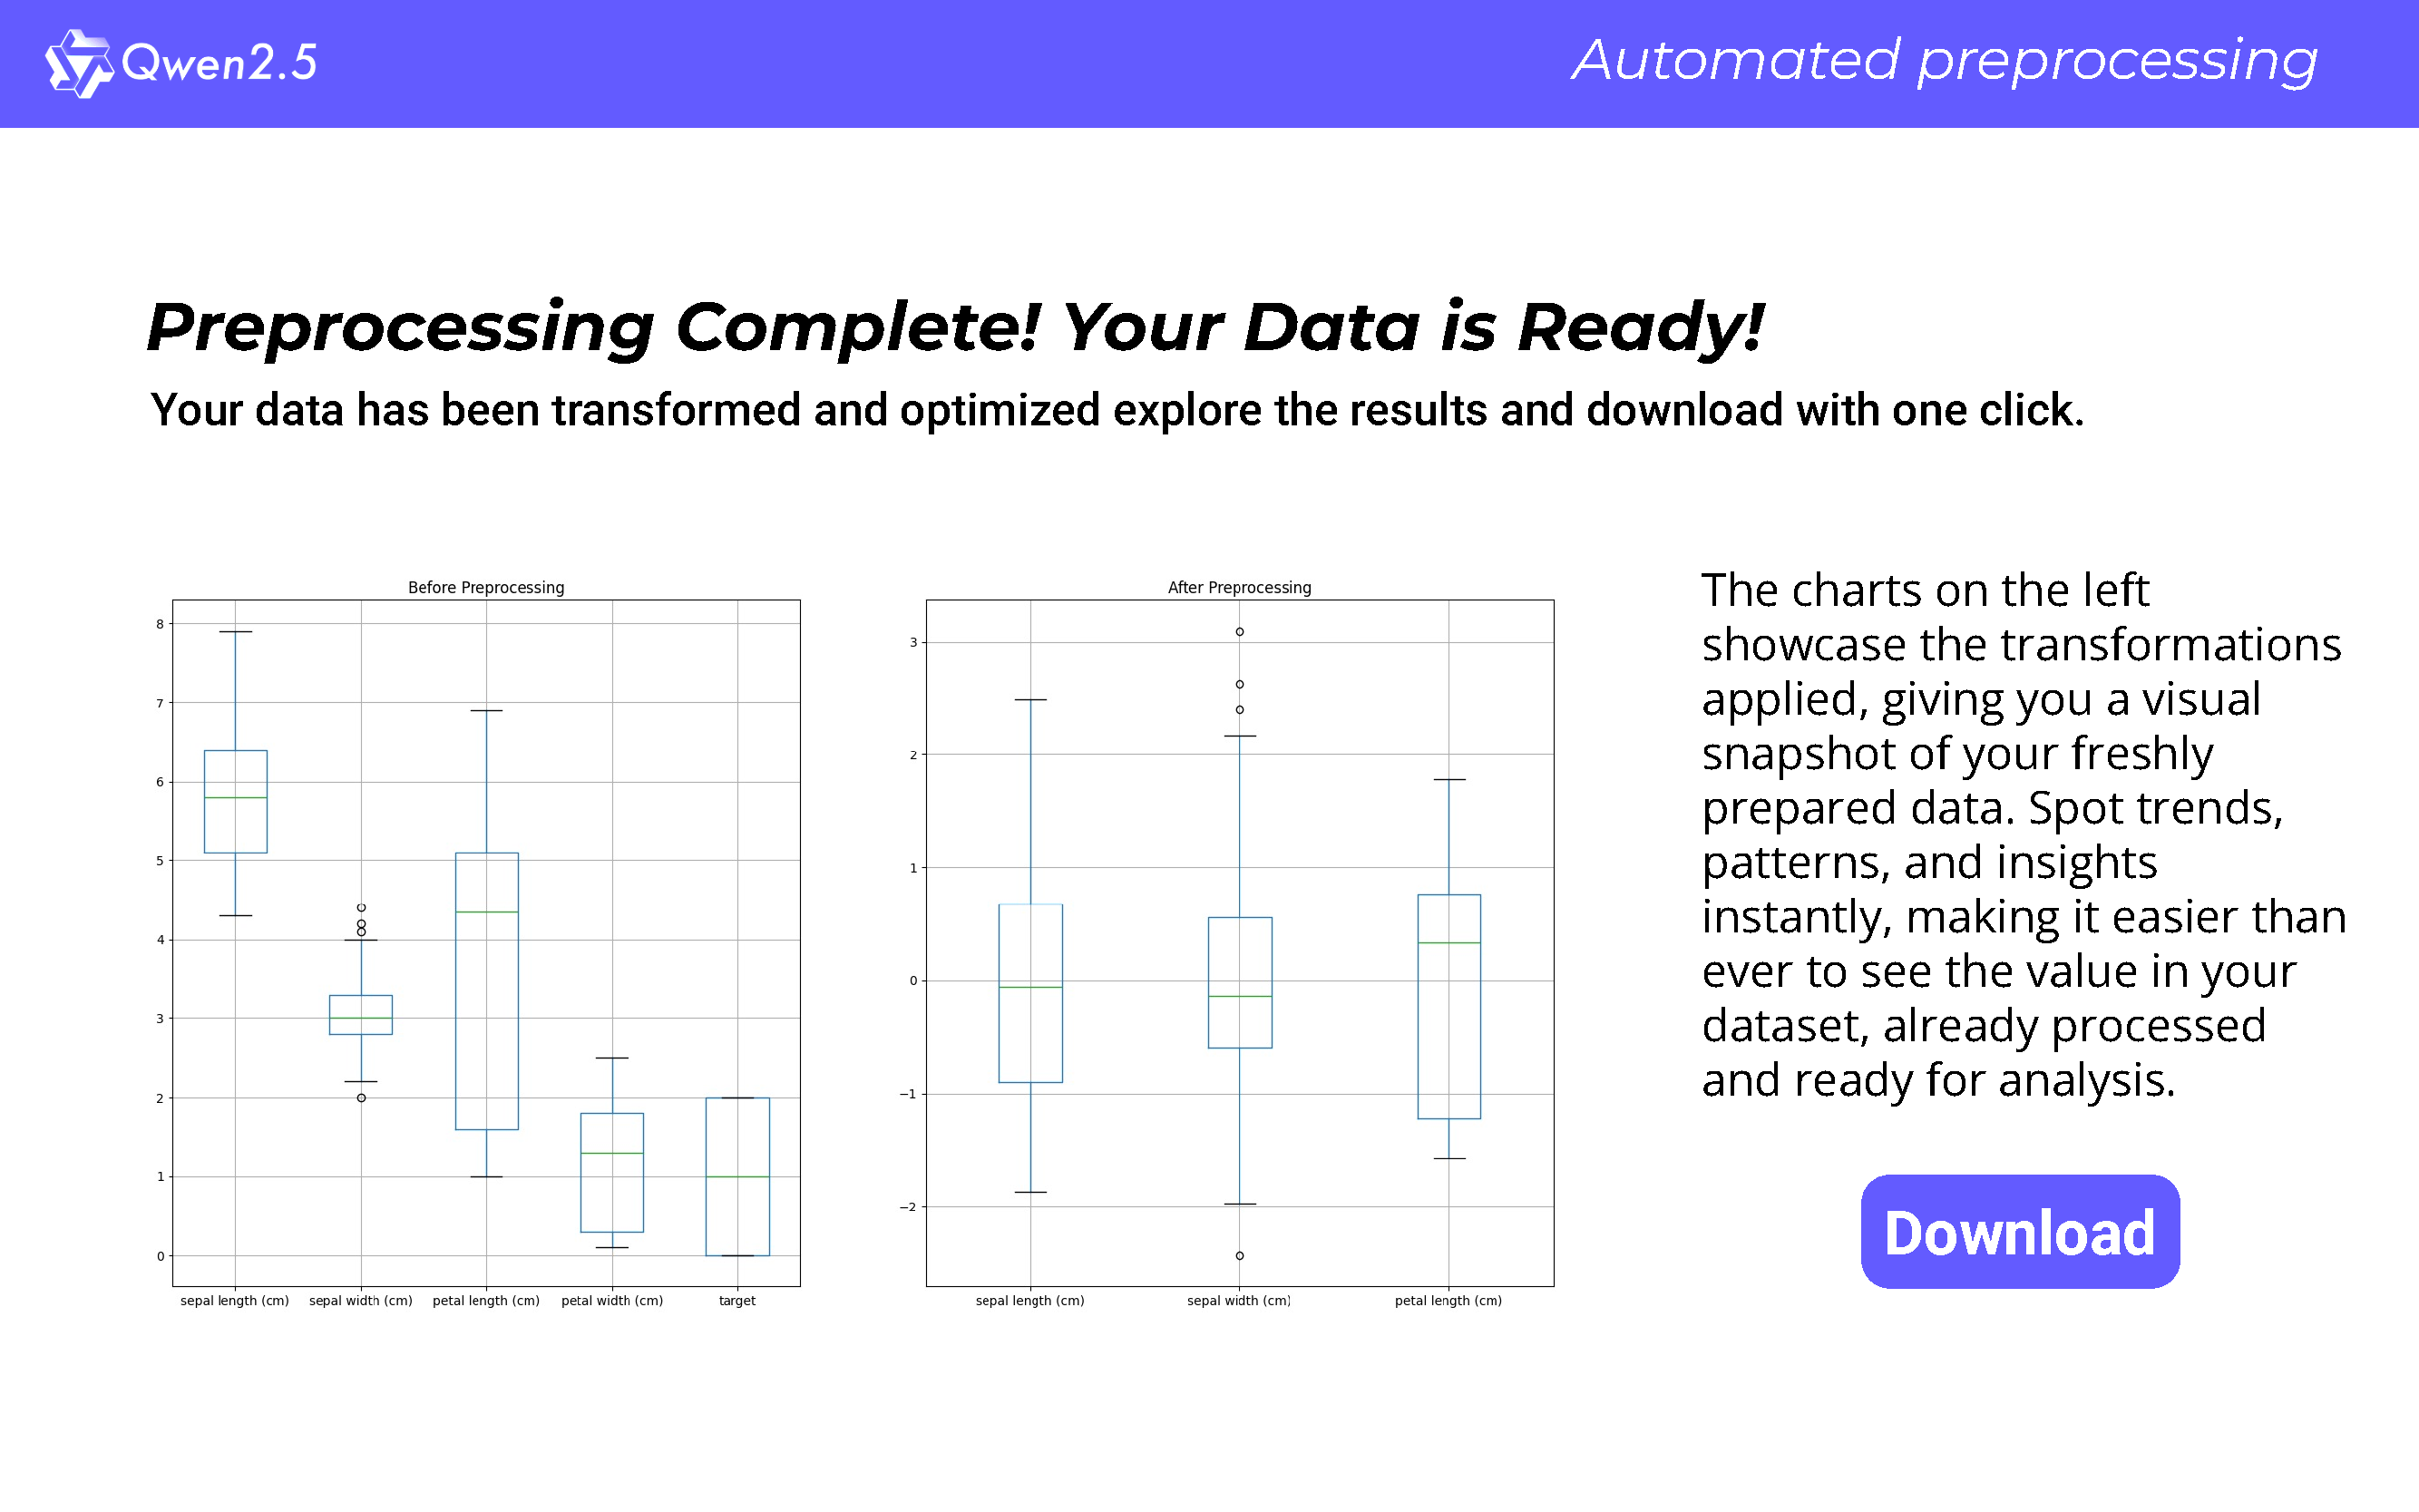
\includegraphics[width=\textwidth]{App_prototipo_2.pdf}
        \caption{Results page of the Qwen2.5 application}
    \end{figure}
\end{frame}

% New Slide: Results and Comparative Analysis
\begin{frame}{Results and Comparative Analysis}
    \textbf{\textcolor{myBlue}{Key Findings and Comparative Insights}}
    \vspace{0.3cm}
    \begin{itemize}
        \item \textbf{Performance Comparison}: Qwen2.5 vs. manual approaches and LLama.
        \item \textbf{\textcolor{myAccent}{Preprocessing Time Reduction}}: Qwen2.5 automates tasks, achieving up to faster dataset cleaning avoiding the time spent on reasoning and decision-making.
        \item \textbf{\textcolor{myAccent}{Consistency and Scalability}}:
            \begin{itemize}
                \item Qwen2.5 demonstrated robust performance on standardized preprocessing tasks.
                \item Limitations emerged with complex datasets, showing need for iterative improvements.
            \end{itemize}
        \item \textbf{Future Potential}: Highlights of Qwen2.5's scalable applications and integration in larger workflows.
    \end{itemize}
\end{frame}

\begin{frame}{Preprocessing Comparison}
    \textbf{\textcolor{myBlue}{Preprocessing Approaches}}
    \vspace{0.3cm}
    \begin{itemize}
        \item \textbf{Comparison of Approaches}:
            \begin{itemize}
                \item Manual preprocessing (our team, Kaggle) vs. automated approaches (Qwen2.5 and LLama3).
            \end{itemize}
        \item \textbf{Qwen2.5 Performance}:
            \begin{itemize}
                \item Outperforms LLama3 with higher accuracy and consistency.
                \item Requires less human intervention but still trails manual methods on complex datasets.
                \item Shows strong performance on small datasets (e.g., Iris), indicating potential for lightweight applications.
                \item Poor performance respect to manual preprocessing on complex datasets,.
            \end{itemize}
    \end{itemize}
\end{frame}

\begin{frame}
    \begin{figure}
        \centering
        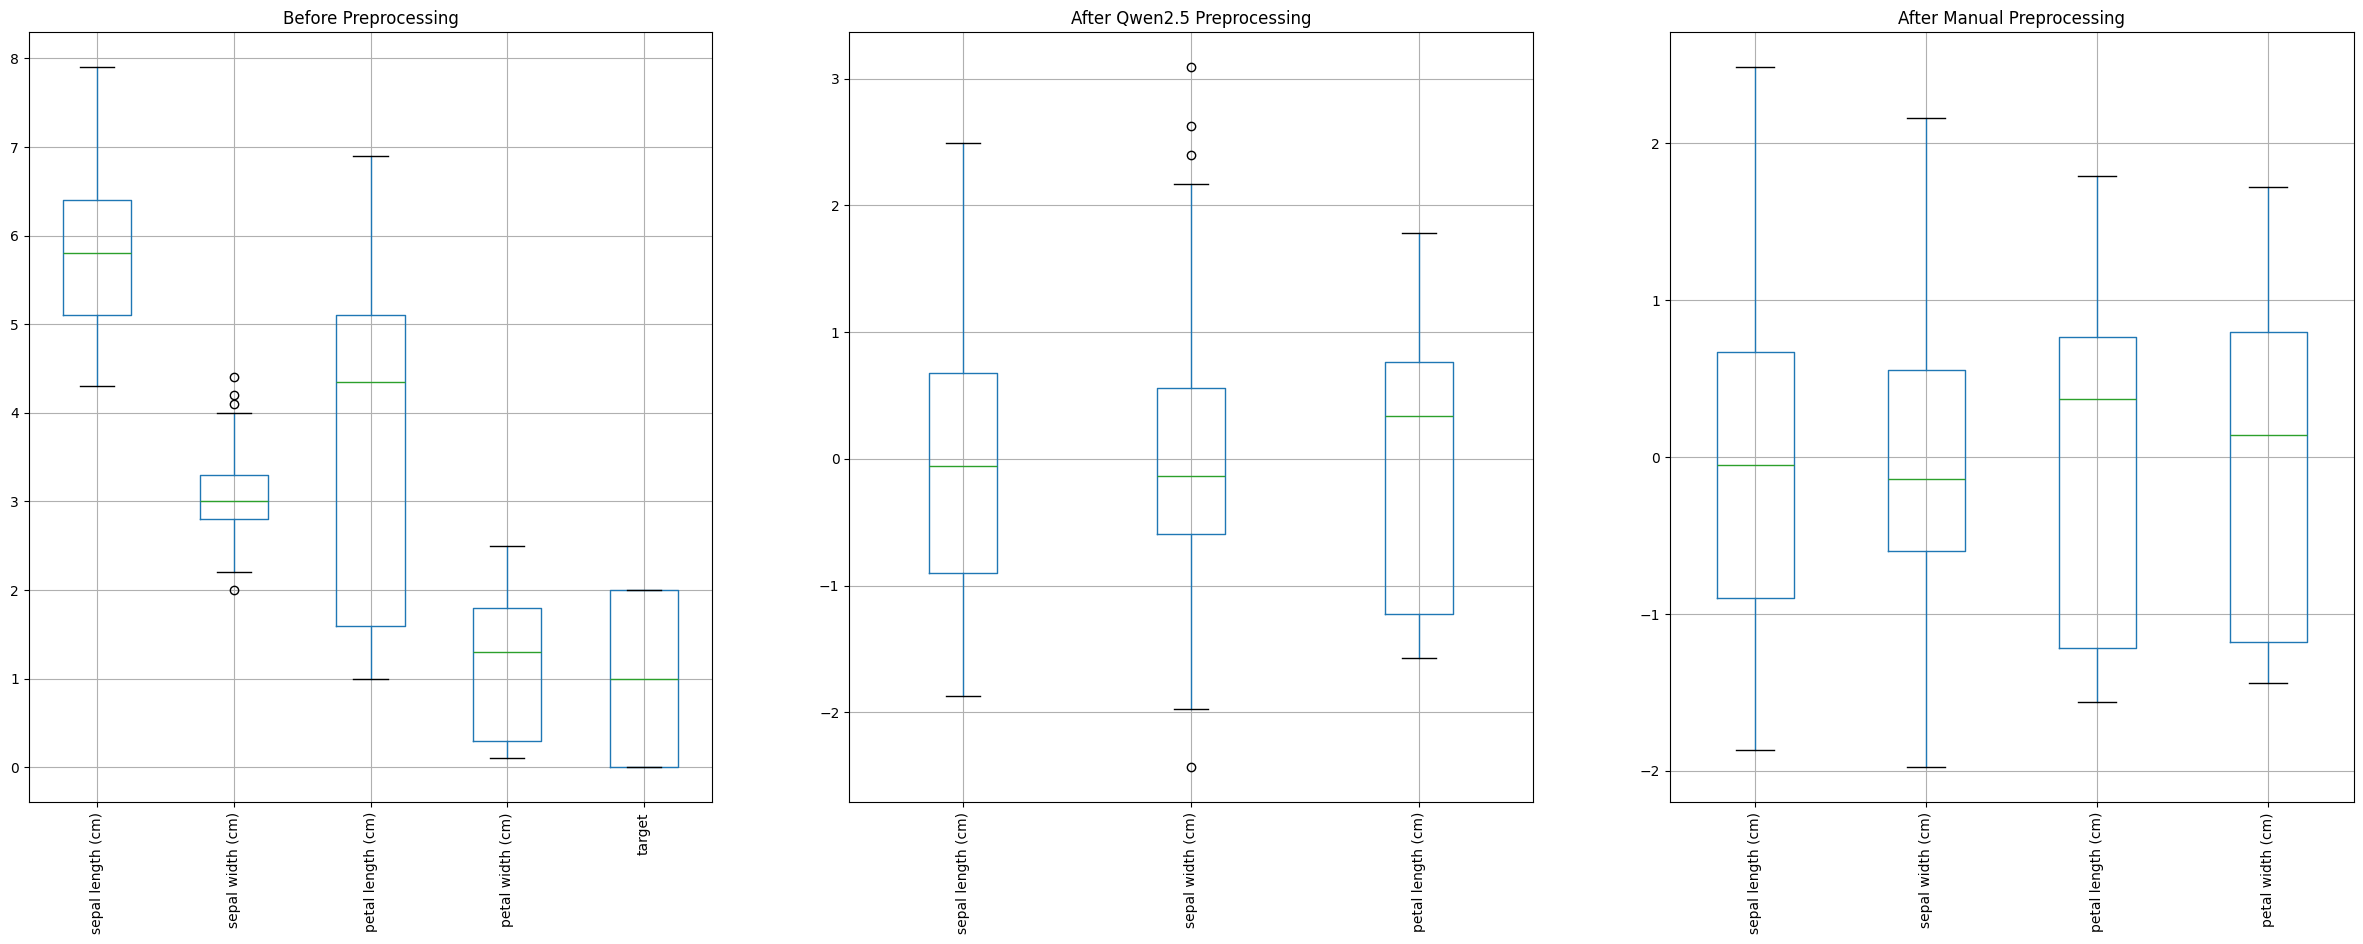
\includegraphics[width=\textwidth]{comparison_iris_with_manual.png}
        \caption{Preprocessing Comparison on Iris Dataset}
    \end{figure}
\end{frame}

\begin{frame}
    \begin{figure}
        \centering
        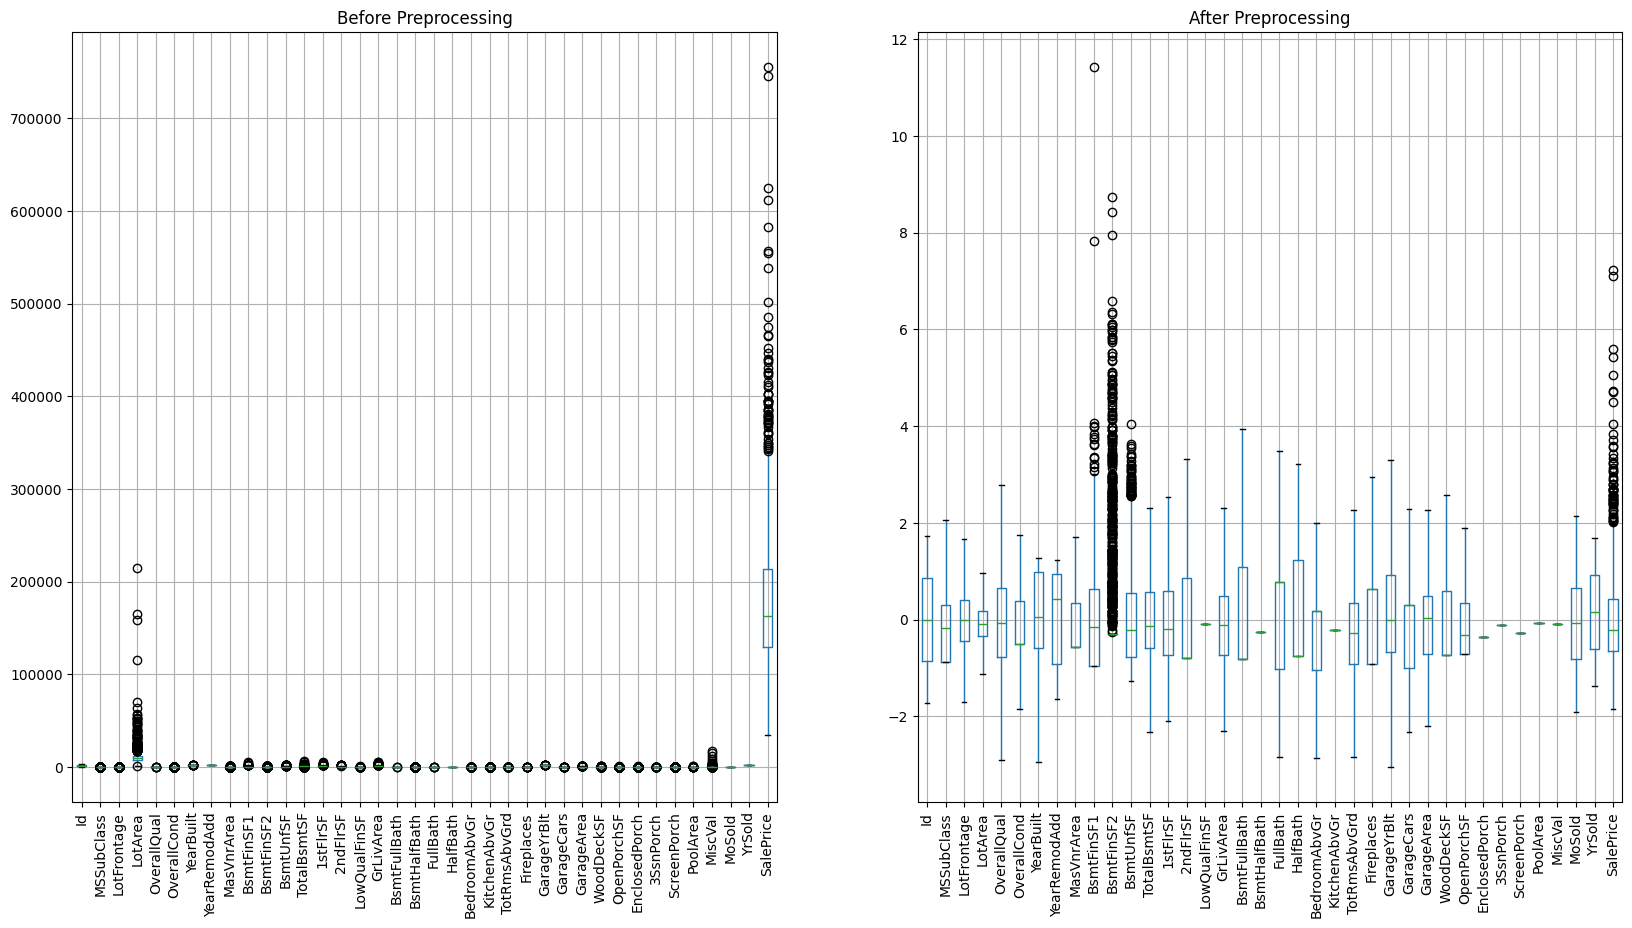
\includegraphics[width=\textwidth]{comparison_house_prices.png}
        \caption{Preprocessing on House Prices Dataset}
    \end{figure}
\end{frame}


% Conclusions
\begin{frame}{Conclusions}
    \textbf{\textcolor{myBlue}{Outcomes}}
    \vspace{0.2cm}
    \begin{itemize}
        \item The experiment demonstrated that Qwen2.5 can automate preprocessing for simple datasets, saving time and costs. However, improvements are needed for handling more complex data, as results in this area were less promising. 
        \item It also highlighted the potential of using LLMs like Qwen2.5 for automating preprocessing, offering businesses a way to reduce the time spent on data preparation, improve efficiency, and allow data professionals to focus on more strategic tasks.
    \end{itemize}
\end{frame}

% Conclusions
\begin{frame}{Conclusions}
    \textbf{\textcolor{myBlue}{Future Potential}}
    \vspace{0.3cm}
    \begin{itemize}
        \item \textbf{Next Steps for Business Integration}: 
            \begin{itemize}
                \item Fine-tuning the model to support even more complex business use cases.
                \item Scaling the solution to handle larger datasets and more diverse business applications.
                \item Continuous improvement through feedback loops, optimizing for business efficiency and accuracy.
                \item Delevoping an iterative approach to improve the model's performance on complex datasets.
                \item Integration of the automated preprocessing system into existing business workflows.
            \end{itemize}
    \end{itemize}
\end{frame}

% Final slide: Thank You
\begin{frame}{Thank You}
    \begin{center}
        \fontsize{20pt}{24pt}\selectfont\textbf{\textcolor{myBlue}{Thank You for your attention!}}\\
        \vspace{0.6cm}
        
        \fontsize{14pt}{18pt}\selectfont\textbf{\textcolor{myAccent}{Feel free to ask any questions}}\\
        \fontsize{14pt}{18pt}\selectfont\textbf{\textcolor{myAccent}{or share your feedback.}}\\
        \vspace{0.6cm}
        
        \fontsize{8pt}{11pt}\selectfont
        \textcolor{myBlue}{f.messina16@studenti.unipi.it}\\
        \textcolor{myBlue}{f.nocella1@studenti.unipi.it}\\
        \textcolor{myBlue}{n.cherchi@studenti.unipi.it}
    \end{center}
\end{frame}

\end{document}
